\section{Does the Checked Policy Improve the Complete Query?}
\label{sec:results}
All 36 main configurations and 16 follow-up policies completed. Figure~\ref{fig:primary} summarizes the primary matrix.\begin{figure*}[!t]
\centering
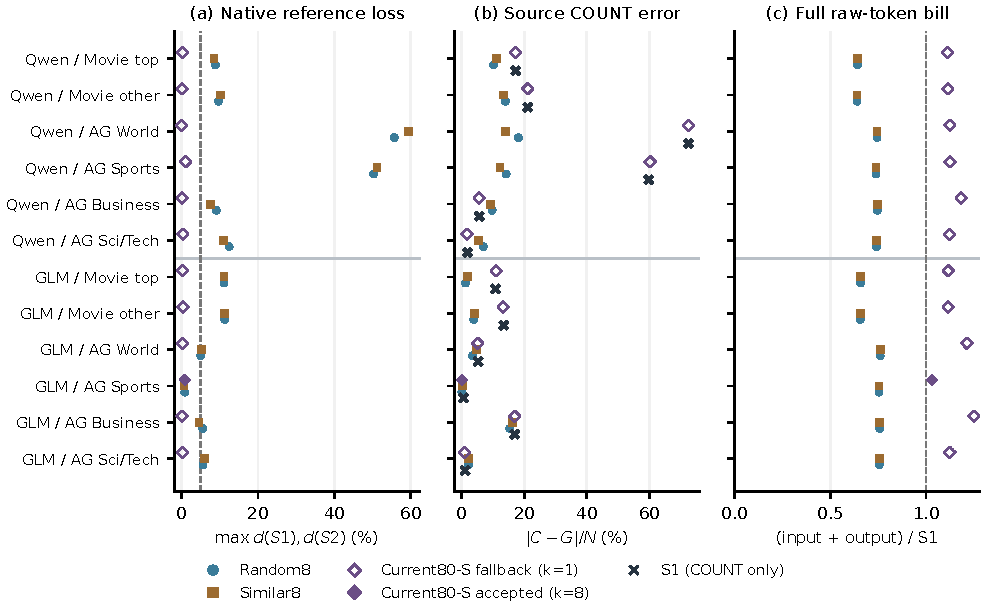
\includegraphics[width=\textwidth]{primary_execution_readouts.pdf}
\caption{All 12 primary configurations ($N=2,048$, cache ON), grouped by model. From left to right: the 0--5\% detail and full range of maximum disagreement with S1/S2; absolute source COUNT error divided by $N$; and complete input-plus-output tokens divided by S1. Smaller values are better. Dashed lines mark the 5\% reference threshold and unit cost. The two fidelity panels show the same measurements at different scales. Hollow diamonds denote fresh singleton fallback; only the filled diamond is an accepted batch. Crosses show S1's source COUNT error.}
\label{fig:primary}
\end{figure*}
 The main checker selected a batch size above one only for GLM Sports at $N=2,048$, cache ON. We follow that execution from checking to the returned count and full bill before examining the remaining outcomes.

\subsection{Walkthrough: A Passed Check and Its Full Bill}
\label{sec:sports_walkthrough}
For GLM Sports, Current80-S selected $k=8$ after all 80 calibration comparisons agreed. The separately seeded validation then found two mismatches in 80 fresh comparisons (2.5\%). Deployment labeled all 2,048 rows in 256 disjoint batches and disagreed with each complete S1/S2 reference on 17 rows (.83\%). The 80/80 checking result, the 2/80 validation result and the 17/2,048 deployment result answer separate questions. Validation is evaluation-only; it changes neither selection nor the policy bill.

The returned count was 519 against source $G=517$, giving $e_N=.10\%$ and $e_G=.39\%$, with 1.66\% source row error, as worked through in Section~\ref{sec:objects}. S1 itself had 2,025/2,048 correct source labels. This provides a usable-reference case for separating fidelity from cost. The separately executed Similar8 plan had 13/2,048 reference mismatches (.63\%); its changed grouping is an observed alternative, not an additional certificate from random probes.

Deployment alone used 256 requests and 255,425 raw input-plus-output tokens. Calibration added 160 requests and 93,120 tokens. The complete policy thus used 416 requests and 348,545 tokens, compared with S1's 2,048 requests and 338,365 tokens. Requests fell by 79.69\%, but raw tokens rose by 3.01\%. The separately executed Random8 baseline had the same observed deployment-only token bill, .754880 times S1. Charging the check consumes that saving, so the checked plan fails the joint benefit criterion despite meeting observed fidelity tolerance.

\subsection{Whole-Policy Benefit Across the Primary Matrix}
\label{sec:bill_results}
Figure~\ref{fig:primary} separates native-reference loss, source COUNT error and full raw-token cost for all 12 primary configurations. Table~\ref{tab:policy_summary} applies the fixed-denominator joint benefit criterion from Section~\ref{sec:resources}. Random8 meets both reference-loss thresholds and lowers requests and raw tokens in GLM Sports (1/12). Similar8 does so in GLM Sports and Business (2/12); Business's maximum reference loss is 4.54\%. These fixed plans have neither calibration cost nor a fidelity certificate.

\begin{table*}[!t]
\centering\tableformat
\caption{Policy comparison over the same 12 primary configurations. Benefit requires a complete result, batching, at most 5\% disagreement with both references, and fewer calls and raw tokens than S1 (Section~\ref{sec:resources}). Cost ratios use each case's S1. Strict benefit keeps all 12 cases; missing complete strict plan/reference vectors are unavailable. The fixed plans' six unavailable cases lack strict references. Source accuracy is evaluated separately.}
\label{tab:policy_summary}
\begin{tabular}{lrrrrr}
\toprule
\tablehead{Plan} & \tablehead{Max. reference loss (\%)} & \tablehead{Calls/S1} & \tablehead{Raw tokens/S1} & \tablehead{Native benefit} & \tablehead{\shortstack{Strict benefit;\\unavailable of 12}} \\
\midrule
Random8 & 0.83--55.71 & 0.125--0.125 & 0.640--0.761 & 1/12 & 1/12; 6 \\
Similar8 & 0.63--59.47 & 0.125--0.125 & 0.640--0.761 & 2/12 & 1/12; 6 \\
Current80-S & 0.00--1.12 & 0.203--1.102 & 1.030--1.251 & 0/12 & 0/12; 6 \\
\bottomrule
\end{tabular}
\end{table*}



Current80-S meets the criterion in 0/12 primary configurations, including 0/10 outside the two Qwen workloads with severe default-True parsing. The other 35 main configurations select fresh singleton fallback and pay for calibration as well as their new complete execution. No secondary size/cache configuration adds a non-singleton selection. Sports was not a preselected scale anchor, so these measurements do not identify its break-even size outside $N=2,048$.

\subsection{Reference Fidelity and Source COUNT Are Different}
\label{sec:quality_results}
The supplied labels also let us evaluate the singleton reference itself; complete per-workload baseline readouts are retained in the artifact. Qwen World and Sports triggered default-True parsing on 1,936 and 1,664 of 2,048 rows. Their native counts were 1,999 versus source $G=514$, and 1,741 versus $G=517$; source row errors were 74.37\% and 60.74\%. A post-hoc World S1 inspection found normal \texttt{stop} termination on all 2,048 calls with only 4--6 output tokens. These observations characterize the frozen two-step query wording, model and native parser together; no matched rewrite isolates the cause. Strict-format checking exposes the format issue while native COUNT remains delivered. Preserving such a reference would also preserve its task errors.

\begin{table*}[!t]
\centering\small
\caption{All 12 primary Current80-S executions ($N=2,048$, cache ON). Every case returns a native COUNT. The two count columns are integers, not a ratio. Strict-valid rows report output format; maximum reference loss compares the native result with both S1/S2. Requests and raw input-plus-output tokens include checking and full execution, divided by S1. Size one denotes fresh singleton fallback.}
\label{tab:primary_results}
\begin{tabular}{lrrrrrrr}
\toprule
Workload & $k$ & \shortstack{Strict-valid\\rows / $N$} & \shortstack{Returned\\COUNT $C_b$} & \shortstack{Source\\COUNT $G$} & \shortstack{Max. reference\\loss (\%)} & Requests/S1 & \shortstack{Raw tokens\\/ S1} \\
\midrule
\multicolumn{8}{l}{\textit{Qwen}} \\
Movie top & 1 & 2048/2,048 & 896 & 1,251 & 0.20 & 1.062 & 1.11 \\
Movie other & 1 & 2048/2,048 & 986 & 1,418 & 0.15 & 1.062 & 1.11 \\
AG World & 1 & 114/2,048 & 1,999 & 514 & 0.00 & 1.062 & 1.12 \\
AG Sports & 1 & 387/2,048 & 1,750 & 517 & 1.12 & 1.062 & 1.12 \\
AG Business & 1 & 2040/2,048 & 613 & 498 & 0.15 & 1.078 & 1.18 \\
AG Sci/Tech & 1 & 2025/2,048 & 483 & 519 & 0.34 & 1.062 & 1.12 \\
\midrule
\multicolumn{8}{l}{\textit{GLM}} \\
Movie top & 1 & 2048/2,048 & 1,025 & 1,251 & 0.24 & 1.062 & 1.12 \\
Movie other & 1 & 2048/2,048 & 1,145 & 1,418 & 0.39 & 1.062 & 1.12 \\
AG World & 1 & 2045/2,048 & 621 & 514 & 0.24 & 1.086 & 1.21 \\
AG Sports & 8 & 2048/2,048 & 519 & 517 & 0.83 & 0.203 & 1.03 \\
AG Business & 1 & 2045/2,048 & 845 & 498 & 0.10 & 1.102 & 1.25 \\
AG Sci/Tech & 1 & 2048/2,048 & 499 & 519 & 0.15 & 1.062 & 1.12 \\
\bottomrule
\end{tabular}
\end{table*}


All 12 primary Current80-S policies delivered native counts, but only six had complete strict vectors (Table~\ref{tab:primary_results}). The native joint benefit result is 0/12. The strict-vector sensitivity has zero satisfied, six evaluated-negative and six unavailable cases. Unavailable strict COUNT is distinct from native query failure.

The unchanged SemBench Q3 integration case illustrates the denominator distinction. Its 2,000-row demonstration relation sends $N=120$ rows to the semantic filter, with $G=14$. Qwen returns 7 and GLM 9 under both cache settings, without defaults and with complete strict outputs. The absolute COUNT errors are seven and five rows: $e_N=5.83\%$ and 4.17\%, but $e_G=50.00\%$ and 35.71\%. These integration measurements are separate from the larger prepared-relation variants.

\subsection{More Probes, the Same Fallback Decisions}
\label{sec:budget_results}
The follow-up holds the native-Boolean agreement rule fixed while comparing Current80-N with Current320-N. All 16 policies select singleton fallback and deliver native COUNT. Twelve have complete strict vectors; four have unavailable strict counts. Table~\ref{tab:budget_results} gives every paired comparison, and Fig.~\ref{fig:budget} separates checking from execution.

\begin{table*}[t]
\centering\small
\caption{Every paired Current80-N$\to$Current320-N follow-up ($N=7,600$, cache ON). $R$: complete requests; $d_{\max}$: maximum native row disagreement with S1/S2. Raw-token and uncached-input ratios compare complete 320-probe with 80-probe policies. Repeats are descriptive; each budget has its own nominal scope.}
\label{tab:budget_results}
\begin{tabular}{llrrrrrr}
\toprule
Model / workload & Rep. & $k$ & \shortstack{Calibration\\calls} & Full $R$ & \shortstack{Raw tokens\\$320/80$} & \shortstack{Uncached input\\$320/80$} & $d_{\max}$ (\%) \\
\midrule
Qwen / AG Sci/Tech & 1 & 1$\to$1 & 160$\to$608 & 7,760$\to$8,208 & 1.11 & 1.13 & 0.41$\to$0.36 \\
Qwen / AG Sci/Tech & 2 & 1$\to$1 & 144$\to$656 & 7,744$\to$8,256 & 1.11 & 1.12 & 0.45$\to$0.28 \\
Qwen / Movie other & 1 & 1$\to$1 & 128$\to$464 & 7,728$\to$8,064 & 1.07 & 1.09 & 0.17$\to$0.17 \\
Qwen / Movie other & 2 & 1$\to$1 & 144$\to$640 & 7,744$\to$8,240 & 1.12 & 1.17 & 0.14$\to$0.20 \\
GLM / AG Sci/Tech & 1 & 1$\to$1 & 176$\to$672 & 7,776$\to$8,272 & 1.16 & 1.21 & 0.16$\to$0.05 \\
GLM / AG Sci/Tech & 2 & 1$\to$1 & 144$\to$736 & 7,744$\to$8,336 & 1.19 & 1.25 & 0.09$\to$0.08 \\
GLM / Movie other & 1 & 1$\to$1 & 128$\to$464 & 7,728$\to$8,064 & 1.07 & 1.10 & 0.20$\to$0.20 \\
GLM / Movie other & 2 & 1$\to$1 & 176$\to$672 & 7,776$\to$8,272 & 1.15 & 1.23 & 0.20$\to$0.14 \\
\bottomrule
\end{tabular}
\end{table*}

\begin{figure*}[!t]
\centering
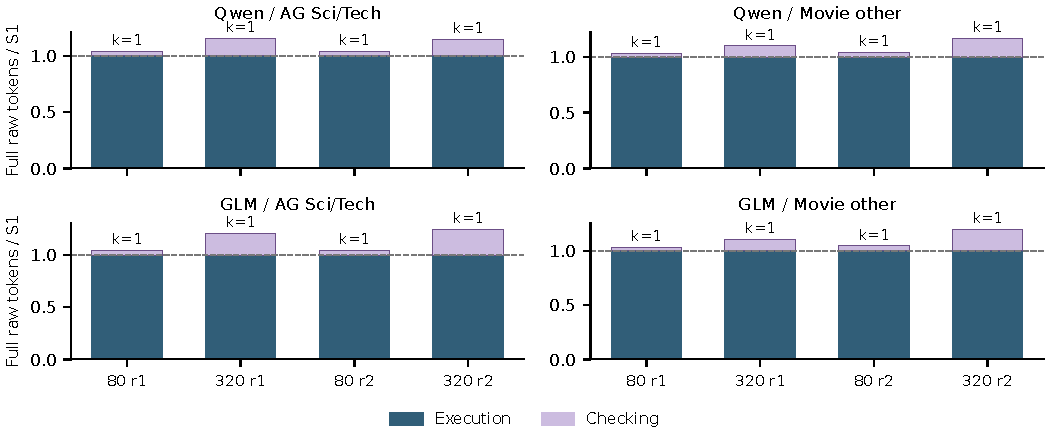
\includegraphics[width=\textwidth]{budget_full_bill.pdf}
\caption{All 16 native-rule follow-up policies ($N=7,600$, cache ON). Each pair compares 80 and 320 probes within one descriptive physical repeat. Bars include fresh calibration and complete execution, divided by the original S1 input-plus-output token bill for that input. Numbers above the bars give total cost ratios; 80 and 320 are probe budgets. Blue denotes execution and violet denotes checking. Every selected size is one. These measured costs are distinct from the hypothetical IID acceptance-power calculation.}
\label{fig:budget}
\end{figure*}

In all eight pairs, 320 probes increase full requests by 4.35--7.64\%, raw tokens by 6.82--19.20\%, and API uncached input by 8.69--25.46\%. Neither tested budget improves the deployment choice on these anchors. The hypothetical IID power calculation in Section~\ref{sec:budget} does not estimate this panel's mismatch probability. Rejecting a candidate means that the policy did not certify it, not that every possible batch is unsafe.

One recorded Qwen AG Sci/Tech pair shows where the extra requests arise ($N=7,600$, cache ON, repeat~1). At budget 80, the three candidates issue 16, 16 and 48 batch probes; the 80 singleton references are reused across them. Checking therefore costs $80+16+16+48=160$ requests. At budget 320 it costs $320+48+112+128=608$. Both policies then obtain 7,600 fresh singleton labels. Table~\ref{tab:budget_worked_pair} places this request arithmetic next to the exact token receipts. In the 80-probe first candidate, the first failure is at trial 14, but the issued 16-request chunk is fully scored and billed; detailed stopping prefixes remain in the artifact.

\begin{table}[t]
\centering\small
\caption{One measured Qwen AG Sci/Tech pair ($N=7,600$, cache ON, repeat 1). Top: requests, with probes listed at sizes 8/4/2. Each full policy adds 7,600 singleton execution calls to checking. Bottom: complete token receipts; $P$ is raw input, $O$ output, $K$ cached input and $U=P-K$.}
\label{tab:budget_worked_pair}
\begin{tabular}{rrrrr}
\toprule
Budget & \shortstack{Singleton\\references} & \shortstack{Batch probes\\8 / 4 / 2} & \shortstack{Checking\\calls} & \shortstack{Full\\calls} \\
\midrule
80 & 80 & 16 / 16 / 48 & 160 & 7,760 \\
320 & 320 & 48 / 112 / 128 & 608 & 8,208 \\
\bottomrule
\end{tabular}
\par\smallskip
\begin{tabular}{rrrrr}
\toprule
Budget & $P$ & $O$ & $K$ & $U$ \\
\midrule
80 & 1,336,641 & 32,108 & 498,816 & 837,825 \\
320 & 1,483,830 & 36,842 & 533,440 & 950,390 \\
\bottomrule
\end{tabular}
\end{table}


The retained stopping-audit CSV records every observed candidate prefix. The main study observes 106 candidate prefixes (105 rejections, one pass); the follow-up observes 48 rejections. At every rejected candidate prefix, accumulated native-Boolean mismatches alone make passing impossible. Qwen also has 31 probe-level strict-only format flags, classified after excluding batch failures and native mismatches. These flags do not mean that format alone caused a candidate stop. No issued probe has a batch-contract failure. The two lower candidates after the Sports pass remain unobserved. Stopped prefixes estimate neither population mismatch probability nor a false-rejection rate.


\subsection{Cache Counters Reverse the Input-Cost Ranking}
\label{sec:cache_results}
All 48 cache-ON fixed-plan executions (24 configurations, two plans) use less raw input but more API uncached input than their own S1. Qwen's ratios are .626--.739 for raw input versus 1.083--1.157 for uncached input; GLM's are .649--.758 versus 1.142--1.285. All 24 cache-OFF fixed-plan executions favor batching on both counters. Table~\ref{tab:cache_costs} keeps raw input, output and uncached input separate, while Fig.~\ref{fig:cache} shows matched examples.

\begin{figure*}[!t]
\centering
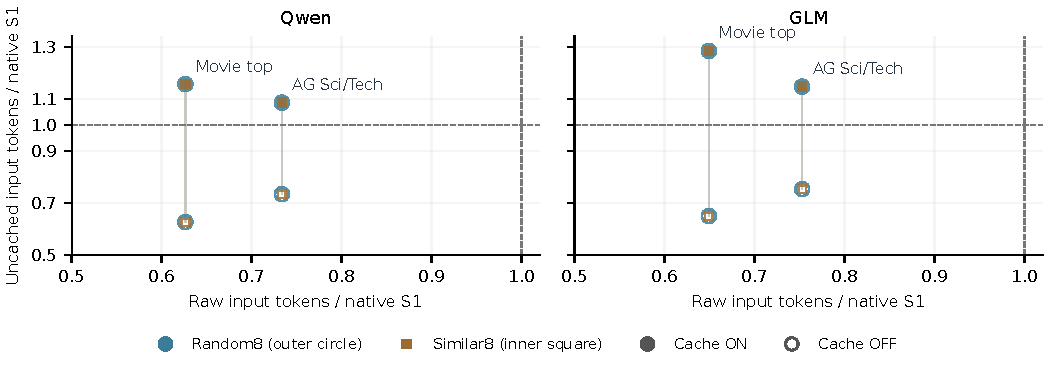
\includegraphics[width=\textwidth]{cache_input_cost_objects.pdf}
\caption{Raw versus API uncached input for Movie top and AG Sci/Tech at $N=7,600$. Lines connect matched cache-OFF/ON executions under each model. Ratios use the corresponding singleton S1 counter; one marks equal cost. Blue Random8 circles and orange Similar8 squares show coincident counters without jitter. Filled markers denote cache ON; hollow markers denote cache OFF. The upper shaded region has fewer raw input tokens but more uncached input than S1. Complete-matrix ranges are in Table~\ref{tab:cache_costs}. Uncached input is a prefill-work proxy.}
\label{fig:cache}
\end{figure*}
\begin{table*}[!t]
\centering\tableformat
\caption{Fixed-plan cost ratios to the corresponding separately executed S1. Cells give complete-matrix ranges; ON has 12 and OFF six configurations per model/plan. The last column counts raw-input ratio $P/P_{S1}<1$ but uncached-input ratio $U/U_{S1}>1$. Input, output and uncached input are distinct; uncached input is a prefill-work proxy.}
\label{tab:cache_costs}
\begin{tabular}{llrrrrr}
\toprule
\tablehead{Model/cache} & \tablehead{Plan} & \tablehead{Cases} & \multicolumn{3}{c}{\tablehead{Cost ratio to singleton S1}} & \tablehead{Reversals} \\
\cmidrule(lr){4-6}
 & & & \tablehead{Raw input} & \tablehead{Output} & \tablehead{Uncached input} & \shortstack{$P/P_{S1}<1$,\\$U/U_{S1}>1$} \\
\midrule
Qwen/ON & Random8 & 12 & 0.63--0.74 & 0.98--1.11 & 1.08--1.16 & 12/12 \\
Qwen/ON & Similar8 & 12 & 0.63--0.74 & 0.97--1.09 & 1.08--1.16 & 12/12 \\
Qwen/OFF & Random8 & 6 & 0.63--0.73 & 1.06--1.08 & 0.63--0.73 & 0/6 \\
Qwen/OFF & Similar8 & 6 & 0.63--0.73 & 1.06--1.08 & 0.63--0.73 & 0/6 \\
\midrule
GLM/ON & Random8 & 12 & 0.65--0.76 & 0.85--0.85 & 1.14--1.28 & 12/12 \\
GLM/ON & Similar8 & 12 & 0.65--0.76 & 0.85--0.85 & 1.14--1.28 & 12/12 \\
GLM/OFF & Random8 & 6 & 0.65--0.75 & 0.85--0.85 & 0.65--0.75 & 0/6 \\
GLM/OFF & Similar8 & 6 & 0.65--0.75 & 0.85--0.85 & 0.65--0.75 & 0/6 \\
\bottomrule
\end{tabular}
\end{table*}


All 24 matched anchor/size/model/fixed-plan comparisons have identical raw input counts with cache ON and OFF. In the running cache-ON Sports case, S1 writes 328,125 input tokens and reuses 131,008, leaving $U=197,117$. Random8 writes fewer inputs (246,721) but reuses only 20,400, leaving $U=226,321$. Its smaller prompt total therefore requires more uncached input. This comparison concerns input processing; the complete raw-token bill also includes output tokens. Output ratios remain separate: .974--1.106 for Qwen and approximately .850 for GLM with cache ON. These are counter rankings for the declared representation, not universal time or monetary advantages.

